\ylDisplay{Projektor} % Ülesande nimi
{Tundmatu autor} % Autor
{lõppvoor} % Voor
{2013} % Aasta
{P 9} % Ülesande nr.
{3} % Raskustase
{
% Teema: Valgusõpetus
\ifStatement
Kodukinoprojektori paigutamisel võib tekkida olukord, kus kujutis tekib ekraani suhtes liiga kõrgele või madalale. Kui üritada kujutist projektori kallutamisega õigesse kohta nihutada, siis venib see trapetsikujuliseks. Mõned projektorid võimaldavad kujutise asukohta siiski ilma moonutusi tekitamata ristsuunas liigutada. Selleks nihutatakse projektori objektiivi optilise peateljega ristuvas suunas, jättes kõik ülejäänud detailid paigale. Vaatame lihtsat projektorit, mis koosneb kumerläätsest fookuskaugusega $f = 60$ $mm$ ja sellest teatud kaugusele paigutatud minikuvarist. Lääts tekitab endast $4L = 4$ $m$ kaugusele paigutatud ekraanile minikuvari terava suurendatud kujutise. Kui palju ja mis suunas tuleb läätse liigutada, et kujutis nihkuks ekraanil $\triangle$$Y$ = $20$ cm võrra kõrgemale?
\fi
\ifHint
Lihtsam on alguses vaadata olukorda, kus lääts on paigal ja liigutatakse minikuvarit. Suurendatud tõelise kujutise tekkimiseks peab minikuvar painema läätsest kaugusel, mis jääb ühe ja kahe fookuskauguse vahele.
\fi
\ifSolution
\begin{center}
	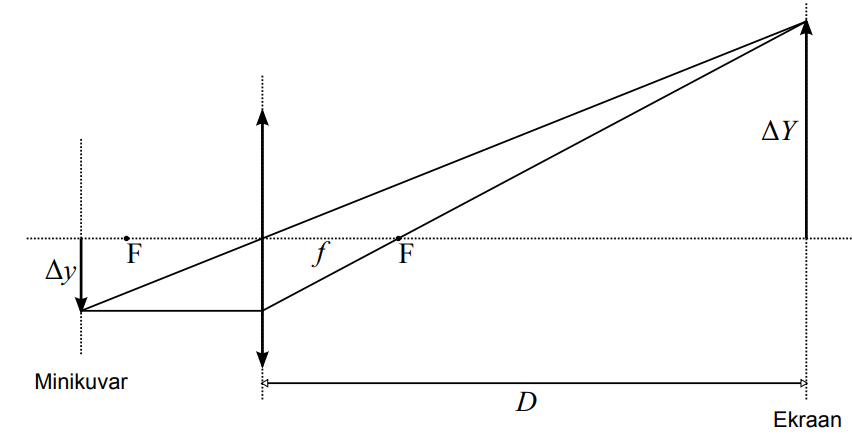
\includegraphics[width=0.5\linewidth]{2013-v3p-09-lah.PNG}
\end{center}
Lihtsam on vaadata olukorda, kus lääts on paigal ja liigutatakse minikuvarit. Suurendatud tõelise kujutise tekkimiseks peab minikuvar painema läätsest kaugusel, mis jääb ühe ja kahe fookuskauguse vahele. Teeme optilisest skeemist joonise. Nihkugu minikuvari mingi punkt läätse suhtes vahemaa $\triangle y$ võrra. Nihet kujutame joonisel noolekesega. Lihtsuse huvides asugu vaadeldav punkt enne nihutamist optilisel peateljel. Konstrueerime kujutise vastava nihke, mille pikkus on $\triangle Y$. Sarnastest kolmnurkadest näeme, et
\begin{center}
$\cfrac {\triangle Y }{\triangle y} =  \cfrac {D - f}{f}$
\end{center}
Tuletame nüüd meelde, et minikuvari asemel nihutame tegelikult läätse. Kui liigutasime minikuvarit läätse suhtes alla, siis nihkus kujutis üles. Sama olukorra kohta võime öelda, et liigutasime läätse minikuvari suhtes üles. See tähendab, et läätse liigutamisel mingis suunas liigub ka kujutis samas suunas. Seetõttu avaldub kujutise kogunihe ekraanil läätse suhtes leitud nihke $\triangle Y$ ja läätse enda nihke $\triangle y$ summana 
\begin{center}
$\triangle Y_kogu = \triangle Y + \triangle y = \cfrac{D - f}{f} \cdot \triangle y + \triangle y = \cfrac{D - f + f}{f} \triangle y = \cfrac{D}{f} \triangle y$. 
\end{center}
Kui kasutada algandmete arvväärtusi, siis saame vastuseks, et kujutise tõstmiseks $20$ $cm$ võrra tuleb läätse nihutada ulespoole $\triangle y = 3$ mm võrra. 
\fi
}